\documentclass[12pt,letterpaper]{article}
%\usepackage{psfig}
\usepackage{amsmath, amssymb}
\usepackage{fullpage}
\usepackage{graphicx}
\usepackage{hyperref}
\setcounter{page}{1}
\pagenumbering{arabic}
\def\pp{\par\noindent}

%%%%%%%%%%%%%%%%%%%%%%%%%%%%%%%%%%%%%%%%%%%%%%%%%%%%%%%%%%%%%%%%%%%%%%%%%%%%%%

\renewcommand{\baselinestretch}{1.2}
\newcommand{\problem}[2]{ \bigskip \pp \textbf{Problem #1}\par}
\newcommand{\problempts}[2]{ \bigskip \pp \textbf{Problem #1} [#2 points]\par}
\newcommand{\itempts}[1]{\item ~~~[{#1}]~~~}
\newcommand{\solution}{\textit{Solution:}\par}
\newcommand{\partA}[1]{ \medskip \pp \emph{Part #1}\par}

%%%%%%%%%%%%%%%%%%%%%%%%%%%%%%%%%%%%%%%%%%%%%%%%%%%%%%%%%%%%%%%%%%%%%%%%%%%%%%

\newcommand{\bbZ}    {\mathbb{Z}}
\newcommand{\bbQ}    {\mathbb{Q}}
\newcommand{\bbN}    {\mathbb{N}}
\newcommand{\bbB}    {\mathbb{B}}
\newcommand{\bbR}    {\mathbb{R}}
\newcommand{\bbC}    {\mathbb{C}}
\newcommand{\calP}   {{\cal{P}}}

\newcommand{\zn}{{\bf 0}_n}
\newcommand{\on}{{\bf 1}_n}

%%%%%%%%%%%%%%%%%%%%%%%%%%%%%%%%%%%%%%%%%%%%%%%%%%%%%%%%%%%%%%%%%%%%%%%%%%%%%%
\begin{document}

\title{Course Search \\ \large{COS435: Final Project}}
\author{David Bieber, Abbi Ward}
\date{May 15, 2012}

\null  % Empty line
\nointerlineskip  % No skip for prev line
\vfill
\let\snewpage \newpage
\let\newpage \relax
\maketitle
\let \newpage \snewpage
\vfill 
\break % page break

\newpage
%%%%%%%%%%%%%%%%%%%%%%%%%%%%%%%%%%%%%%%%%%%%%%%%%

\begin{abstract}
The purpose of this project is to create an application specific search engine for the purpose of finding Princeton courses highly relevant to any course information need.
The resulting search engine takes simple text queries, and returns a list of courses relevant to the query. The project includes a crawler for gather the course data from the Princeton Registrar's website, as well as all of the components of the search engine, which is built on top of Lucene.
The search engine built for this project performs better than and handles more types of queries than either of the two existing alternatives, the Integrated Course Engine (ICE) and the Registrar's own search feature.
\end{abstract}

\section{Introduction}
We created a robust Princeton course search engine. It handles free-text queries and can be integrated with the ICE (Integrated Course Engine) application that many students use for scheduling.
In addition to allowing users to search for specific courses, it allows users to get P/D/F-able and P/D/F only courses and search and filter based on the amount of reading per week required and the professors teaching the course, in addition to other course information.
The search engine is built on top of Apache Lucene, an open source Java search engine library. Lucene helps manage the index and parse queries into acceptable formats.
As part of creating the search engine, we built a scraper tool that scrapes the Registrar's Course Offerings page and stores all course data.

\section{Goals}
Our motivation for this project stems from our own need to find courses to take at Princeton. There are already a few ways to look for classes including the paper course catalog, word of mouth, the Registrar's website, and the Integrated Course Engine (ICE).
Each method offers its own advantages but still students complain about the difficulties of searching for desired courses. Given a course, these tools provide the relevant information about it. However, if we start with an information need we cannot easily find a course that satisfies it.
In particular, students often request the ability to search for P/D/F-able or P/D/F-only classes, classes with light reading, or classes of a particular difficulty. Additionally, students frequently have time constraints that limit what courses they may choose from, and there is no existing convenient way to search within these contraints.
	
We set out to create a tool to satisfy these demands. The search engine we set out to make must satisfy three objectives. It must be \emph{simpler than the registrar's search feature}, which is clunky in the sense that search requires entering exact match values for specific fields.
It must be \emph{more flexible than ICE}, which is missing the ability to search by critical course information like professor and reading material. And it must be \emph{more powerful than either} of the two, as they both lack the ability to search for information students find useful, such as P/D/F options, amount of reading, and course difficulty.
The existing tools also lack the ability to flexibly combine search constraints. Neither ICE nor the registrar allows you to search for both keywords and time of day simulatenously, for instance.
	
For our search engine, we aimed to create a single free text search box that can handle all of a student's course informaion needs. In particular, our search engine must allow students to find P/D/F-able classes, classes of a desired reading amount, classes about a particular topic, and classes that fit their schedule. It also must allow students to combine these search contraints freely, and it must provide the courses the student is most likely interested in first.
	
\section{Features}

\subsection{User facing}
\begin{enumerate}
\item Free text search. One search bar for everything.
  
  The user can simply put what they want into the search bar (for instance, a pdf-able class on Tuesday at 1:30) and they'll get back courses that fit or nearly fit that description. The search is natural and requires little thought from the user on formulating his information need. 
  
\item Basic Search Capabilities
  
  Our search engine can perform the same capabilities as the Registrar's search and ICE, combined. Given a course title, department, professor, keywords or any other basic information about the course, our engine will return relevant results. There are no restrictions on how a user can combine search constraints.
  
\item PDF and Audit Options
  
  The user can easily search for P/D/F-able, non P/D/F-able, or P/D/F-only classes, as well as auditable, or non-auditable classes.
  
\item Time and Day
			  
  The user can specify the time and day of the courses for which they're looking. The search engine prioritizes courses that take place in those time slots.
  
\item Reading per week
  
  The user may specify a desired amount of reading per week. The search engine returns courses with reading amounts in that range. For this and all of our features, the user may specify their search in a human readable format. The search engine will do its best to understand ``100 pages per week'' or ``100 pp/wk'', for instance.
  
\end{enumerate}

\subsection{Additional Features}
\begin{enumerate}
\item Scraping registrar
  
  We've created a tool that scrapes the registrar and stores all course data in an easily accessible data format. It is resistant to registrar server failures, as well as local failures.
			
\item Updating index
  
  The Indexer interprets our course data and creates an inverted index. As new courses become available or new data becomes available about old courses, the index is updated to reflect these changes.
  
\end{enumerate}

\section{Use Cases}
\subsection{Max the Lazy Architect}
Max is interested in art and architecture, and really hates all forms of work. He'd love to sleep in until noon, and he'd like to take the easiest classes possible. Of course, he needs to fulfill his departmental and distribution requirements, but he doesn't really care how as long as he can take his daily afternoon nap. So Max pulls up our search engine and types in ``easy afternoon courses''. He gets PSY 207. It's an SA distribution, is P/D/F-able, and lectures don't start until 12:30 pm. ``I'll take it!'' he exclaims, then takes a 15 minute Reddit break before looking for more classes. Max decides to look at courses he needs to take for architecture. He first decides to look at ARC and technology through the query 'ARC technology' and sees ARC 311 looks like an interesting course.
		
\subsection{Julie the Undecided Poet}
Julie can't decide between psychology and poetry. She wishes to pursue understanding the abnormalities and idiosyncracies of the human mind, through both art and science. She first browses the psychology offerings through the query 'psy' and decides PSY 207 would be an appropriate course. Julie then, looking for a challenge, seeks a course with about 200 pages of reading per week and no P/D/F option using the query 'ENG 200 pages no p/d/f'.She finds ENG 344, Topics in Romanticism: Romantic Passions, is a perfect fit for her interests.  

\section{Components}

\subsection{Architecture Overview}
Our search engine has several key components that together allow for sophisticated course searches. A visual overview is provided in the accompanying figure. The data that is searchable all comes from the registrar. We crawl pages on the registrar with our Registrar Scraper in order to accumulate this data. The scraper uses application specific logic in order to get a meaningful understanding of information from the HTML pages on the registrar's website. The data is serialized to disk and is used to build the inverted index that our search engine relies upon. Our Indexer, built atop Lucene, maintains the index on disk. When our search engine receives a query, it first applys the query parser in order to create an application specific query. The query parser determines the meaning of the query, so that the search engine knows what to look for in what fields of the indexed course documents. The result of query parsing is then used with the inverted index in order to generate a number of results. These are ranked and given as the result of the search.

\begin{figure}
\begin{center}
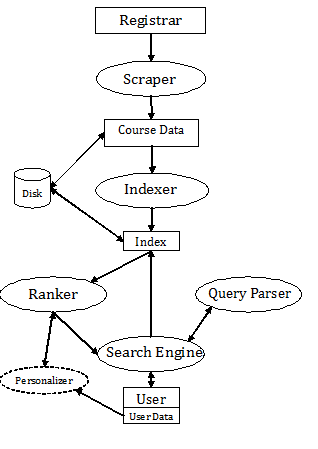
\includegraphics{OverallArchDiagram.png}
\end{center}
\caption{Architecture Overview}
\end{figure}

\subsection{Registrar Scraper}

Our registrar scraper operates in three tiers and is highly specific to the job of scraping course data. A visual overview of the registrar scraper's logic is provided in the accompanying figure. The first tier contains a single document, the registrar's main page, from which we scrape a list of department pages. The second tier is made of these department pages, each of which contains a list of courses. We begin gather course specific information on the second tier, as the department pages contain information about when the classes meet, how large the classes are, and what distribution areas they satisfy. Additionally and most importantly we crawl the second tier for links to pages with additional information about the classes. These class specific pages form the third tier of the registrar scraper. For each page in the third tier we gather as much information as possible about the individual course represented. We can usually find most of the following information about each class: the professor teaching it, a description of the class, a sample reading list, any prerequesites, the way the class is graded, P/D/F and audit options, the amount of work to expect, when the course is offered, and sometimes even more. All of the information about the classes gather during tiers two and three is aggregated and serialized to disk so that it can be later used by the indexer.

The course data for the whole registrar is 1649kB. While scraping the whole registrar, 6 department pages failed to load and 52 course pages failed to load on the first try. Our scraper handled these failures gracefully and reconnected to these pages at a later time. The time of day at which we scrape may be a factor. All but 1 link succeeded on the second iteration. The last one, Macroeconomics/Int'l Finance Workshop, succeeded on the third iteration. There are 1201 total courses and 96 departments (from the perspective of our scraper -- Freshman Seminars and Writing Seminars are considered departments by it). This gives us a $4.3\%$ error rate for courses, $6.3\%$ error rate for department pages, and a $4.5\%$ error rate overall. 

\subsection{Indexer}
	
The indexer takes the RegistrarData object we created in the RegistrarScraper and returns an inverted index. We first take all the course data and put it into documents, one per course. In Lucene, documents consist of sets of fields. We use the key-value pairs from the CourseDetails object of each course as fields in each document. This method of construction allows us to take advantage of the known information structure for user search. Through this application-specific structure, we can parse queries to examine particualr fields and will thus return more accurate results. Furthermore, the parallel structure between CourseDetails object and our Indexer makes the code clear and easy to extend and change. If we expand our project to include additional sources, such as the SCORE evaluations and the Student Course Guide, this extensability is critical. 

We then create the index using a Standard Analyzer which turns our text in the documents into tokens and applies two filters. It first makes everything lowercase, and then it eliminates stop words (such as ``a'', ``an'',  ``and'', ``are'', ``as'', ``at'', ``be'', ``but'', ``by'', ``for'', ``if'', ``in'', ``into'', ``is'', ``it'', ``no'', ``not'', ``of'', ``on'', ``or'', ``such'', ``that'', ``the'', ``their'', ``then'', ``there'', ``these'', ``they'', ``this'', ``to'', ``was'', ``will'', ``with''). We have also configured it to overwrite the index as we update. This means we can update documents without worrying if they'll be indexed twice. At the end of this process, we have created a searchable index that contains all the course information. 

The index of our course data is 370kB, giving a compression ratio of 0.224 with respect to the course data scraped. It indexes our course data in an average of 2.1 seconds. 
	
\subsection{Query Parser}
	
The two primary components of the query parser are our CourseQuery parsing and Lucene's multi-field query parser. From a user's query, we create a CourseQuery object. The CourseQuery object parses this query to extract pdf-options, days, times and reading amount. To extract the P/D/F and audit options information, it searches the query for a pre-determined set of keywords, such as ``pdf'' or ``easy''. It then extracts these from the free-text portion of the query and appends to the remaining query directions for the value the searcher should search. For instance, a query including ``pdf-only art drawing'' will become ``art drawing pdf: only'' at this stage. A similar process occurs for days, times, and reading amount. For times, we perform two special operations. We must convert ranges to sets of values and put these values into military time. We also search for special time search terms such as ``afternoon'' or ``noon'' and use them to set ranges of times. We do not remove these terms from the query in the case that time is not the query term's intention. Once we have extracted the Princeton-specific information, we pass our new query to Lucene's multi-field query parser. This parser takes a query string expands it into a form suitable for searching a Lucene index. Specifically, for each search term for which a field is not specified, it constructs the query such that the searcher will search all specified fields for the term. 
	
\subsection{Search Engine}
At this level, the user types a query into the search bar. The query is sent to the query parser which puts it into a form appropriate for the index. The searcher is a Lucene object created from the index. For a given query, it retrieves information from the index and compiles a list ranked by score. ??? We then take these ranked results and re-order them according to our own ranking scheme. ???

This search engine is a Chrome extension and accompanies the existing ICE tool. Our extension takes over the search bar on ICE and submits queries to our server. 
				
		
\subsection{Ranker}

\subsubsection{Lucene Ranking}
The Lucene ranking takes into account several factors. 
\begin{equation}
  score(q,d) = coord(q,d) * queryNorm * \sum_{\text{term t } \in q}{tf(\text{t in d}) * idf(t)^2 * termBoost(t) * norm(t,d)}
  \label{eq:practical}
\end{equation}
$coord(q,d)$ is the number of terms in doc d\\
$queryNorm$ is a normalizing factor and allows comparison between queries. It is the Euclidean norm of the weights as determined by ???\\
$tf(\text{t in d})$ represents the term frequency of term t in document d \\
$idf(t)$ is the inverse document frequency of term t and is represented mathematically by \[ 1 + log(\frac{numDocs}{docFreq + 1}) \] where docFreq is the frequency of term t in each document. \\
$termBoost(t)$ is a factor that essentially boosts a given term t in query q. For instance, we could boost time and days specified to give classes that fit the user's need better.\\
$norm(t, d)$ takes into account the document boosts (we can boost documents to appear more frequently), lengthNorm (a factor that allows short fields to contribute more to the score), and the individual field boosts for which term t is the name of a field. 
\[ norm(t,d) = docBoost(d) * lengthNorm * \prod_{\text{field f in d named as t}}{fieldBoost(f)} \] 				

\subsubsection{Course Ranking}
At indexing time, we adjusted the fieldBoost for the following fields: course abbreviation, distribution area, title, and PDF. We chose these fields as they tend to be most relevant to a user's query. We determined these values experimentally using a technique similar to the machine learning method gradient descent. As the default fieldBoost values are 1.0, indicating no boost, we first tried our algorithm without any boosting. The results were stellar but the ranking was less than adequate. Based on an educated guess, we set the initial boost values to 1.07

\section{Experiments}

\section{Evaluation}
\subsection{Experiment Testing}
\begin{enumerate}
\item Class specific: ELE 301, ENG 300
\item Department specific: COS, ARC
\item Number specific: 126, 217
\item Professor: Chazelle
\item Course Title: Japanese Society
\item Include PDF: pdfonly art
\end{enumerate}

We are limited in the queries we can use to compare our search engine with the existing ones because the queries ICE and the registrar accept are severely limited compared to the ones our search engine accepts.
\subsection{Experiment Results}

We tested our index without fieldBoosts versus the index with fieldBoosts. As the score is only affected when relevant fields are selected, we chose queries that included those fields. We found that the ranking with the boosts was improved. 

\begin{tabular}{ | l | c | r |}
	
\end{tabular}

\subsection{Comparison with Existing Search Engines}
\begin{enumerate}
\item Registrar Search
  The Registrar Search is essentially a database query. You select values for particular fields and the registrar returns results that exactly match the values for those chosen fields. Results are returned in alphabetical order by course abbreviation. 
  
\item ICE
  From what we can tell based on experimentation, ICE only indexes the description, title, and course abbreviation. It suffices then as a tool to create a schedule but is not, at the moment, a tool that's effective for finding courses to take. ICE does allow you to search by time but not in conjunction with other search terms. The results ICE returns are in alphabetical order by course abbreviation (i.e. COS 435). They are not truly ranked.  
  
\item Conclusion
  None of these search engines give the ability to search for the pdf option and none offers the same flexibility as ours.
\end{enumerate}

\section{Future Works}

\subsection{Personalization}

Personal Data
The following is the personal data we could use to implement personalized search results. These are data we theoretically have access to on the ICE platform.
\begin{enumerate}
\item Course History
\item Associated Ratings for each course taken
\item Friend's Data
\item Search History
\end{enumerate}
What we would do with the data:
\begin{enumerate}
\item Use search history to tailor results

\item Rank higher the departments in which you've taken courses and have high ratings for that department's courses

This would be especially useful for breaking ties. For instance, I'm more interested in ELE 218 than CLA 218 so if I search 218, ELE 218 should be the top result. 

\item Know which prerequisites you've filled and give a warning before adding

\end{enumerate}

	
\subsection{User Interface}
Because our engine takes free-text queries rather than database queries, when we return results they are ranked by best-fit rather than a yes or no. Thus, if the user enters several terms, we may have results that don't exactly satisfy the information need. To help address this from the user's perspective, we could have a display that also lists the relevant fields searched. For instance, if I search ``CLA MW 330 pdfonly'', then in addition to listing CLA XXX - TITLE, the time/days and pdf options would also be displayed. This allows the user to determine at a glance if the search has been satisfied in an acceptable way. 
As we have the scores of document in the returned results list. We could compute a percent match to the query to give the user a sense of expected relevance. We could also implement feedback so that the user could give us a thumbs up for relevant or interesting courses. 

As we hope to fully integrate this with ICE, our primary flexibility is with the ranking order and details per hit. We have already created a Chrome extension that takes over the search bar and can send a request to our own server.  

\subsection{Additional Signals}

There are a variety of other sources we may use to help refine our results. We could use SCORE evaluations and the student course guide to help students choose courses with lighter workloads. Additionally, data on friends's course histories also serve as a ranking signal. We could also consider signals outside ICE such as what's trending on Twitter or on PrincetonFML, a site where students go to complain, celebrate, and share snippets of their lives. 

\section{Conclusion}

We useful tool for Princeton students. In order to create it, we had to learn about web scraping and built our own Princeton-specific web crawler. Towards the end of the project, we moved towards the Mercator model, as we used queues to determine which links to crawl. Our search engine is designed to meet students's information needs. In addition to basic searches, we successfully are able to search for desired PDF and audit options. We can also search for reading amounts and under schedule constraints. We've also created code that is easy to maintain and extend, as we choose to incorporate more signals.


\appendix

\section{Source Code}
\url{https://github.com/dbieber/coursesearch}

\section{Max and Julie}
Max and Julie met in PSY 207. They realized they're both abnormal in very different ways, and they belong together. They lived happily ever after. The End.

\section{Thanks}
Thanks for a great course. Some of our favorite topics were the recommender systems and Map Reduce. Also, we enjoyed the story at the end of the course about the agents that communicate with one another. 

\section{Works Cited}
\subsection{Reference}
\url{http://lucene.apache.org/} \\
\url{jsoup.org} \\
\url{http://www.lucenetutorial.com/sample-apps/textfileindexer-java.html} \\
\url{http://lucene.apache.org/core/old_versioned_docs/versions/3_5_0/api/all/org/apache/lucene/search/Similarity.html} \\
\end{document}
